%!TeX encoding = UTF-8
%!TeX program = xelatex
% --------------------------------------------------------
%  欢迎使用桂林电子科技大学本科毕业论文LaTex模板(v3.0)
%    项目：https://github.com/wrm244/GUEThesis
%     请参考项目目录下的docs文件夹额外说明
%编译指导：请下载MiKTeX软件后，运行根目录下的makefile.bat即可自动编译
% --------------------------------------------------------
\special{dvipdfmx:config z 1}
% 修改数值是否压缩，1：压缩，0：不压缩，不压缩会加快编译速度，但会增加PDF体积

\documentclass[eversion]{thesis-guet} 
% documentclass[]参数：eversion:电子版 pversion:打印版
% \usepackage{showframe} % 显示排版框架
% \TPshowboxestrue % 显示textblock 框架，方便调整位置

\definecolor{shadecolor}{RGB}{255,204,75} % 定义高亮颜色
\graphicspath{{./image/},{./image/2},{./image/4},{./image/chapter1/},{./image/chapter2/}}% 图片所在位置

% ----------------------------------------------
%     文章信息
% ----------------------------------------------
\title{基于RAG的“三高”慢性病医学问答系统设计与实现}{} % 题目{中文}{英文}
\author{牛嘉贺}
\advisor{李优}   % 导师姓名
\protitle{教授}  % 导师职称.
\school{计算机与信息安全学院}  % 所在学院
\major{计算机科学与技术}  % 学科专业或领域
\studentnumber{2200820924}  % 学号
\degreecategories{工学学士}  % 申请学位门类或类别
\datereply{\today}  % 可更换为具体日期如：\datereply{2023年5月28日}

% -----------------------------------------------
%     封面
% -----------------------------------------------
\begin{document}
\makecover % 封面
%也可使用另外添加PDF文件作为封面，如盲审封面 \bindpdfcover{盲审学位论文封面(示例).pdf} 
\originalitydeclaration % 独创性声明
%也可使用已签字的扫面版独创性声明PDF文件 \signatureofdeclaration{./docs/独创性声明(示例).pdf} 
% !Mode:: "TeX:UTF-8"

\begin{chineseabstract}

近年来，随着人口老龄化加剧，高血压、高血糖和高血脂（“三高”）慢性病人群持续扩大，围绕指标监测、用药管理和生活方式干预的日常咨询需求显著增长。传统线下问诊在便利性和及时性方面存在限制，难以满足“三高”患者高频、连续的健康信息获取需求。与此同时，大语言模型在自然语言理解与生成任务中展现出较强能力，为智能医疗问答提供了新的技术路径。

但是，在医学等高风险应用场景中，大语言模型仍存在一定局限，例如会产生事实性错误（幻觉）、安全性约束不足以及专业知识利用不充分。因此，有必要将检索增强生成（Retrieval-Augmented Generation, RAG）与模型优化方法结合，以提升模型在“三高”慢病问答中的安全性与可靠性。

针对上述问题，本文围绕“三高”慢性病咨询场景，设计并实现了基于RAG的医学问答系统。本文首先通过国家政策、学术期刊和临床指南等可靠来源构建医学知识库。考虑到“三高”问答同时存在医学术语精确匹配需求与语义理解需求，单一路径检索难以兼顾召回覆盖与相关性，因此进一步设计了融合关键词检索与语义检索的混合检索策略，为生成阶段提供更稳定的外部证据支撑。针对模型安全性约束不足等问题，本文引入直接偏好优化（Direct Preference Optimization, DPO）方法，基于偏好数据对模型进行优化，使生成内容更符合医学场景下的安全性与规范性要求。在此基础上，本文完成了系统的整体设计与实现，形成了从知识构建、检索增强到答案生成的完整问答流程。

实验结果表明，所提出的混合检索在召回覆盖率上优于单一路径检索，Recall@5达到89\%；同时，基于DPO优化后的模型在盲评中相较基础模型取得59.2\%的胜率，并在事实一致性与回答完备性等指标上表现更优。

\chinesekeyword{检索增强生成；大语言模型；混合检索；直接偏好优化；医学问答系统}
\end{chineseabstract}

\begin{englishabstract}
In recent years, with the acceleration of population aging, the number of patients with hypertension, hyperglycemia, and hyperlipidemia (the "three highs") has continued to increase, and the demand for daily consultations on indicator monitoring, medication management, and lifestyle intervention has grown significantly. Traditional offline consultation is limited in convenience and timeliness, making it difficult to support the high-frequency and continuous information needs in this scenario. Meanwhile, large language models (LLMs) have shown strong capabilities in natural language understanding and generation, providing a new technical path for intelligent medical question answering.

However, in high-risk scenarios such as medicine, LLMs still have notable limitations, including factual hallucinations, insufficient safety constraints, and inadequate use of domain knowledge. Therefore, it is necessary to combine Retrieval-Augmented Generation (RAG) with model optimization methods to improve safety and reliability in the "three highs" medical QA setting.

To address these issues, this paper designs and implements a RAG-based medical question answering system for consultations on "three highs" chronic diseases. A medical knowledge base is first constructed from reliable sources, including national policies, academic literature, and clinical guidelines. Since this task requires both precise medical term matching and semantic understanding, a single retrieval path is often insufficient. Therefore, a hybrid retrieval strategy that combines keyword retrieval and semantic retrieval is proposed to provide more robust external evidence for answer generation. To further improve response safety and quality, Direct Preference Optimization (DPO) is introduced to align model outputs with medical safety and compliance requirements. Based on these methods, the paper completes the full system design and implementation, covering the entire QA pipeline from knowledge construction and retrieval augmentation to answer generation.

Experimental results show that the proposed hybrid retrieval outperforms single-path retrieval in recall coverage, achieving 89\% Recall@5. In addition, the DPO-optimized model achieves a 59.2\% win rate over the base model in blind evaluation, and performs better in factual consistency and answer completeness.

\englishkeyword{Retrieval-Augmented Generation; Large Language Model; Hybrid Retrieval; Direct Preference Optimization; Medical Question Answering System}
\end{englishabstract}
 % 摘要
\thesistableofcontents   % 目录
\thesiscontent
% -------------------------------------------------
%    论文各章节(详见目录下chapter文件夹)
% -------------------------------------------------
\chapter{绪论}

\section{课题的研究背景与意义}

随着人口老龄化不断加深，慢性病管理已成为公共健康领域的长期议题。在常见慢性病中，高血压、高血糖和高血脂患者数量大、管理周期长、复发风险高，患者往往不能只依赖少数几次门诊完成健康管理。与急性疾病不同，慢性病管理更强调日常监测和持续干预，患者在真实生活中会频繁遇到诸如指标是否异常、饮食如何调整、药物需不需要复查、症状是否需要就医等具体问题\cite{ZWSG202601012}。这类问题看似琐碎，却直接影响持续治疗情况和病情控制效果。

传统医疗服务以线下诊疗为主，患者通常只有感到身体不适或按固定的时间安排才会选择就医，患者难以获得持续、及时的健康指导。同时，由于医疗资源分布不均以及医生数量相对有限，患者在非就诊期间获取专业医疗建议的渠道较为有限。所以很多患者选择去互联网搜索相关健康信息，但互联网上信息来源复杂、质量参差不齐，用户很难从中获得可靠的医学建议。

近年来，大语言模型（Large Language Model，LLM）发展很快，在理解和生成文本方面都有明显提升，通过大语言模型构建智能医疗问答系统成为可能。基于LLM的问答系统能够理解用户提出的问题，并生成相对流畅的回答，在医疗咨询等场景中展现出一定应用潜力。但是将通用LLM直接应用在医学领域时，会面临知识更新滞后、事实错误（幻觉）以及缺乏依据等问题\cite{YXQB202601003}。

基于这一背景，本文引入检索增强生成（Retrieval-Augmented Generation，RAG）技术，将外部医学知识库与大语言模型结合起来\cite{Ji_2023}。其核心思路是在模型生成答案前先检索相关医学资料，根据资料组织回答，而不是单纯依靠模型的“记忆”作答。这样做的价值主要体现在三个方面：第一，可以降低医学问答中的幻觉风险；第二，可以让回答建立在可追溯的证据基础上；第三，更便于系统随知识更新而持续维护。因而，围绕“三高”慢病场景研究并实现一套基于RAG的医学问答系统，既具有现实应用意义，也具有一定的技术研究价值。

\section{国内外研究现状}

\subsection{互联网问诊的发展现状}

随着互联网技术和智能手机的普及，互联网问诊模式出现并迅速发展。根据中国互联网络信息中心第56次《中国互联网络发展状况统计报告》显示，截至2025年底，中国网民规模达11.25亿，互联网普及率突破80\%\cite{CNNICReport56_2025}。互联网问诊依托其便捷高效、实时互动、及良好的隐私保护特性等优势，迅速普及，吸引了大量互联网企业、传统医疗机构及新兴在线医疗平台积极参与\cite{WSGL201702004}。目前，国内的互联网医疗代表性平台有微医、好大夫在线、京东健康、平安健康和阿里健康等，其主要提供医生在线问诊、健康信息发布以及购药等服务。这些平台更多是作为传统线下医疗服务的补充形式，在一定程度上提升了患者获取医疗信息的便利性。不过，平台提供的信息质量参差不齐，不同来源之间可能存在内容差异，影响用户判断；在线问诊以人工问答为主，受限于有限的医疗资源，患者还是会面临回复不及时等问题。

国外的医疗平台则更注重于远程医疗。例如，瑞典的KRY和美国Teladoc Health、Doctor on Demand等平台实行线上预约并利用会议视频实时问诊，让患者在家里即可享受到专业的医疗问诊\cite{WRKX201206003}。但这类服务仍有很多不足，首先是患者可能需要支出额外的费用，以享受远程问诊的服务；而且平台签约医生数量相对固定，高峰时段还需预约排队；如果涉及身体检查的情况，仍需要去线下医院就诊。

现阶段互联网问诊仍主要依赖人工医生答复，其服务能力、响应效率和服务成本都受到现实医疗资源的制约。在这一背景下，如何借助自然语言处理与智能问答技术，为用户提供更及时、更稳定的医学信息支持，逐渐成为医学人工智能研究的重要问题，因此也推动了医学问答模型的持续发展。

\subsection{传统医学问答模型的发展现状}

早期医学自然语言处理模型主要集中在医学术语识别、实体抽取和文献理解等任务上，代表性工作包括BioBERT、BlueBERT、ClinicalBERT和PubMedBERT等。这类模型大多建立在BERT框架之上，通过PubMed文献、临床记录或生物医学语料继续预训练，使模型在医学词汇和专业语义建模方面明显优于通用语言模型。其主要价值在于提升医学文本表示能力，为后续问答、分类和关系抽取等任务提供基础，但这类模型主要是以理解任务为主。

随着大模型技术的发展，医学问答研究进一步转向生成式模型。例如，由Google提出的Med-PaLM和Med-PaLM 2模型，Med-PaLM系列模型是专门针对于医学领域的大语言模型，Med-PaLM通过医学领域微调和人工评估，使其在医学考试题、患者咨询和临床推理任务中相较于通用大语言模型有更好的表现，Med-PaLM也是第一个在美国医师执照考试样例问题中获得“合格”的模型\cite{Singhal_2025}。国内的科研机构也在积极推进大模型在医学领域的应用，也推出了许多针对于医学领域的大模型，例如：DoctorGLM、华佗GPT等。DoctorGLM是基于ChatGLM的中文问诊模型，其对通用大语言做了针对医疗领域进行微调与优化工作；香港中文大学和深圳大数据研究院的研究团队推出的华佗GPT-o1，首次将推理能力融入到了医学大模型。

医学问答模型虽然已经从BioBERT、PubMedBERT一类的领域预训练模型发展到Med-PaLM、HuatuoGPT、DISC-MedLLM、MedFound等生成式医学模型，但在真实应用场景中仍存在明显不足。其一，很多模型在考试题或标准问答集上表现较好，但面对日常慢病咨询中的口语化表达、连续追问和个性化问题时，稳定性仍然不足。其二，纯生成式模型往往难以同时满足“回答自然”和“证据清晰”这两个要求，尤其在治疗建议、药物说明和风险判断等问题上更容易暴露安全边界问题。其三，现有研究更多关注模型能力本身，而对知识更新、检索链路、证据展示和系统落地等系统实现环节关注不足。

\section{本文研究内容}

针对“三高”慢性病场景下大语言模型在可信性、安全性以及系统落地方面存在的问题\cite{JYRJ202407001}，本文围绕基于检索增强生成（Retrieval-Augmented Generation, RAG）的医学问答系统展开研究与实现。本文主要工作包括面向垂直医疗场景的关键技术设计以及系统工程实现。

本文的具体研究内容如下：

（1）围绕“三高”相关慢性病主题构建医学知识库，对相关政策文件、临床诊疗指南、健康科普资料以及互联网医学文本等数据进行整理和预处理，并通过文本切分和向量编码等方式，形成适用于检索增强生成框架的结构化知识基础。针对医学文本专业术语密集、信息表达高度压缩以及上下文依赖性较强等特点，重点分析了知识组织方式对后续检索效果与生成质量的影响。

（2）针对医学问答场景中单一检索策略难以同时兼顾精确匹配与语义召回的问题，设计了关键词检索与向量检索相结合的混合检索策略，并引入重排序与结果筛选机制，以提升检索证据的相关性与可靠性。在此基础上，构建基于大语言模型的生成流程，使模型能够结合检索到的外部医学证据进行答案生成，从而在一定程度上提升回答的准确性与可解释性。

（3）设计并实现了一套面向实际应用的医学问答系统，围绕用户问答交互、知识检索服务、模型推理调用以及结果展示等核心模块进行整体架构设计，实现了从知识导入、索引构建到在线问答服务的完整流程。同时，系统支持多轮对话、证据来源展示以及知识库管理等功能，使系统能够较好地服务于实际慢病健康咨询场景。

\section{论文组织结构}

本文共分为六章，各章内容安排如下：

第一章：绪论，介绍课题研究背景与意义，梳理国内外研究现状，并给出本文的研究内容与技术路线。

第二章：相关理论和技术介绍，主要阐述大语言模型、Transformer、检索增强生成（RAG）等基础理论，为后续方法设计提供理论支撑。

第三章：医学知识库构建与检索方法，重点介绍“三高”领域知识库的数据来源、预处理与向量化过程，以及BM25、向量检索与混合检索策略的设计与实验分析。

第四章：医学问答模型构建与优化，围绕RAG问答生成流程、Prompt与上下文构建、DPO偏好数据构造和训练过程展开，并通过实验评估模型优化效果。

第五章：系统设计与实现，从系统需求、总体架构、业务模块、数据库设计、模型推理服务与前端页面等方面，说明医学问答系统的工程实现过程。

第六章：：总结与展望，对全文工作进行归纳，分析当前工作的不足，并给出后续可改进方向。

\chapter{相关理论和技术介绍}

\section{大语言模型概述}

大语言模型（Large Language Models，LLM）是近年来自然语言处理领域最具代表性的技术进展之一。其基本思路是通过大规模文本训练，让模型学习语言中的语法规律、语义关系和上下文依赖。与传统模型相比，大语言模型参数规模更大，能够处理更复杂的语言现象，也因此在问答、对话、摘要和内容生成等任务中表现出更强的泛化能力。当前主流大语言模型大多建立在Transformer框架之上，因此理解Transformer的基本原理，是分析后续RAG系统与模型优化方法的前提。

\subsection{Transformer模型}

Transformer由Vaswani等人在2017年提出\cite{Vaswani_2017_AttentionIsAllYouNeed}，其关键突破在于用自注意力机制替代传统循环结构建模序列关系。与RNN和LSTM相比，Transformer不需要按时间步逐次处理输入，因此训练并行度更高，也更容易捕捉长距离依赖关系。这两个特点直接推动了其在大规模预训练中的广泛应用。

\begin{figure}[htb]
    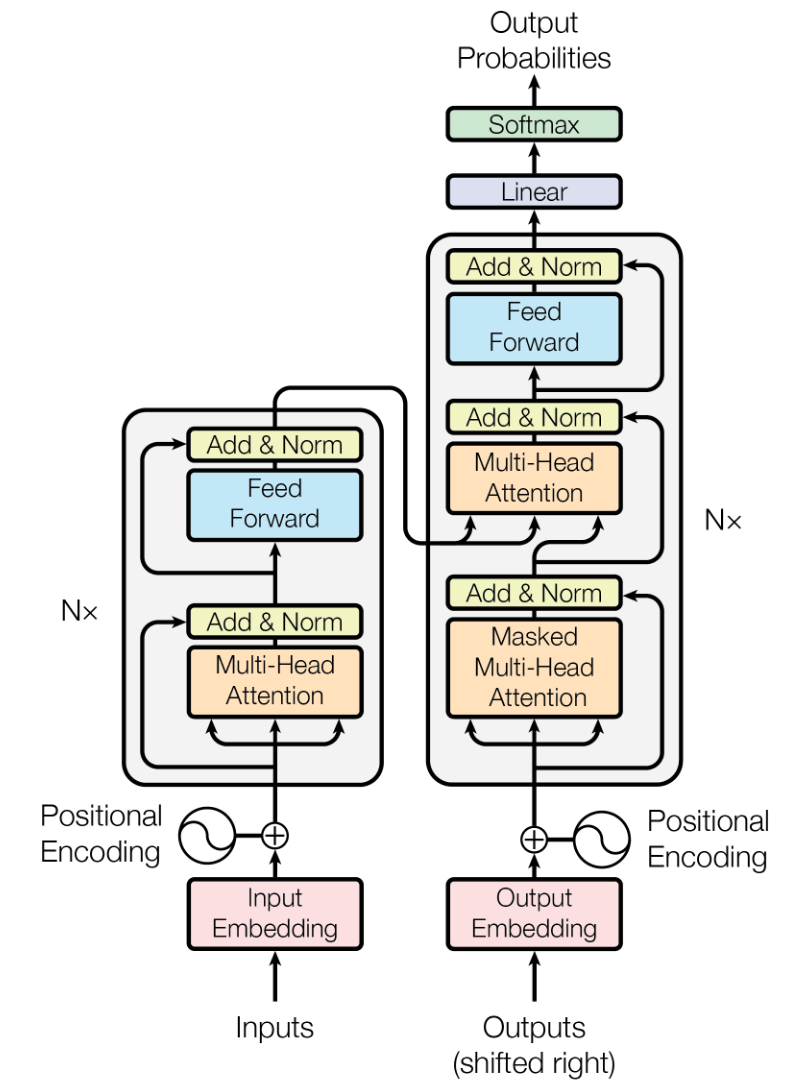
\includegraphics[width=0.5 \textwidth]{image/2/transformer1.png}
    \caption{Transformer结构图}
    \label{fig:transformer-structure}
\end{figure}

如图\ref{fig:transformer-structure}所示，Transformer由编码器和解码器两部分组成。编码器负责将输入序列转换为高维语义表示，解码器则依据这些表示逐步生成输出。编码器和解码器都由多层重复堆叠构成，其中最核心的模块是多头自注意力和前馈神经网络。为了提升训练稳定性，模型还在各子层后加入残差连接和归一化操作。解码器与编码器相比，多了掩码自注意力和编码器-解码器注意力，用于保证生成过程满足自回归约束，并充分利用输入语义信息。

自注意力机制是Transformer的核心。它的作用不是简单地“看上下文”，而是根据当前词与序列中其他词之间的相关性，动态分配信息权重。具体来说，输入向量会被映射为查询（Query）、键（Key）和值（Value）三个表示，再通过Query与Key的相似度计算注意力分数，并对Value加权求和，形成新的上下文表示。其标准形式为：
\begin{equation}
Attention(Q, K, V) = softmax(\frac{QK^T}{\sqrt{d_k}})V
\end{equation}
其中，$Q$、$K$、$V$分别表示查询、键和值矩阵，$d_k$表示键向量维度。分母中的缩放项用于避免点积过大，减轻softmax进入梯度饱和区的问题。进一步地，多头注意力将这一过程并行执行多次，使模型能够从不同表示子空间观察同一段文本，从而提高特征表达能力。

\subsection{现代大模型}

现代大语言模型虽然仍然建立在Transformer的基本思想之上，但在结构设计上已经不再完全沿用最初的Encoder-Decoder框架。当前主流模型，如GPT、LLaMA和Qwen，大多采用仅解码器（Decoder-only）结构。这种结构更适合自回归生成任务，因为模型在训练时和实际生成时都遵循相近的过程，也就是根据已有上下文去预测下一个词元。

在具体实现上，现代大模型围绕训练稳定性、长上下文建模能力和推理效率做了很多改进。先看归一化方式，不少模型已经从Post-Norm转向Pre-Norm，也就是先做归一化，再进入注意力层和前馈层，这样更有利于缓解深层网络中的梯度传播问题。有些模型还会使用RMSNorm替代LayerNorm，用来减少一部分计算开销。再看位置编码，旋转位置编码（RoPE）已经成为比较主流的做法，和绝对位置编码相比，它更适合处理长距离依赖，在长文本理解和多轮对话场景中通常也更稳定。

此外，现代大模型也对前馈网络和注意力实现做了更有针对性的优化。例如，在前馈层中加入SwiGLU这类门控结构，可以在参数规模接近的情况下提升非线性表达能力；在注意力机制里，采用多查询注意力（MQA）或分组查询注意力（GQA）能够减少KV Cache占用，减轻推理阶段的显存压力。对于长上下文推理，更高效的FlashAttention则从实现层面降低了显存读写开销。它不会显式保存完整的注意力矩阵，而是把$Q$、$K$、$V$按块处理，并在片上缓存中完成局部计算和在线归一化，从而在保持结果等价的同时明显提升效率。其等价形式可以写作
\begin{equation}
 y_i = \sum_j \frac{\exp \left(q_i \cdot \frac{k_j}{\sqrt{d}} \right)}{\sum_l \exp \left(q_i \cdot \frac{k_l}{\sqrt{d}} \right)} v_j
\end{equation}

总体来看，现代大模型的这些改进并不是简单叠加出来的，而是围绕“大规模训练能够顺利进行”和“长上下文推理能够保持效率”这两个目标逐步形成的一条技术路线，这也为后续RAG系统在复杂问答场景中的应用提供了模型基础。

\subsection{模型训练技术}

大语言模型能力的形成，通常会经历预训练、监督微调和偏好优化等阶段。预训练阶段依赖大量无标注文本，通过下一词预测等自监督任务学习通用语言规律，这一阶段会决定模型最基础的理解和生成能力。对于通用任务来说，预训练模型往往已经具备较强能力，但在医学问答这类垂直场景中，只依靠通用能力通常还不够，因为领域术语理解、回答风格控制和安全边界把握都需要更有针对性的训练。

监督微调（Supervised Fine-Tuning，SFT）是最常见的任务适配方式，它利用“输入-输出”标注样本，让模型学习特定任务中的回答形式和表达方式。对医学问答来说，SFT的价值不只是提高回答正确率，更重要的是帮助模型学会更符合医学场景的组织结构，比如先回答核心问题，再补充解释和风险提示。

不过，随着模型规模不断增大，全参数微调的成本也越来越高。基于这一点，参数高效微调（PEFT）方法被越来越广泛地采用，其中LoRA是比较常见的一类。LoRA通过在原有权重矩阵上加入低秩增量参数，实现“只更新少量参数、主体权重基本保持冻结”的训练方式，这样既能明显降低显存开销和部署成本，也更适合论文系统实现中算力条件有限的情况。

在监督微调之后，模型虽然已经学会了“按要求作答”，但未必真正知道“什么样的回答更好”。为了进一步提升输出质量，研究者提出了基于人类反馈的强化学习（RLHF）方法。RLHF一般会先利用人工偏好数据训练奖励模型，再借助强化学习算法优化生成模型，使输出结果更接近人类偏好。不过，这一流程涉及奖励建模、策略优化和训练稳定性控制，整体链路较长，实现起来也更复杂。

为简化偏好学习过程，2023年提出的直接偏好优化（Direct Preference Optimization，DPO）提供了一条更直接的实现路径。DPO不再单独训练奖励模型，而是直接利用“优选回答-非优选回答”这类成对数据来优化模型偏好。其目标函数可以表示为
\begin{equation}
\mathcal{L}_{DPO}(\theta) = - \mathbb{E}_{(x, y_w, y_l) \sim \mathcal{D}}
\left[
\log \sigma
\left(
\beta \log \frac{\pi_{\theta}(y_w|x)}{\pi_{ref}(y_w|x)}
- \beta \log \frac{\pi_{\theta}(y_l|x)}{\pi_{ref}(y_l|x)}
\right)
\right]
\end{equation}
其中，$x$表示输入问题，$y_w$表示优选回答，$y_l$表示非优选回答，$\pi_{\theta}$表示待优化模型，$\pi_{ref}$表示参考模型，$\beta$表示偏好强度参数。这个目标的含义比较直接，就是在同一个输入条件下，提高模型生成优选回答的相对概率，降低模型生成非优选回答的相对概率。对于医学问答场景来说，这种方法特别适合用来强化审慎表达、结构清楚和安全提示较充分这类输出偏好。

\section{检索增强生成（RAG）技术}

检索增强生成（Retrieval-Augmented Generation，RAG）是一种将信息检索与文本生成结合起来的方法。它的出发点并不复杂：大语言模型虽然具备很强的语言组织能力，但其知识主要固化在训练参数中，面对专业问题或新近知识时，仍可能出现遗漏和误答。RAG的作用，就是在模型生成前先从外部知识库中检索相关内容，再把这些内容作为上下文交给模型使用。

从流程上看，RAG通常包含“检索”和“生成”两个核心环节。系统先根据用户问题构造查询，从知识库中召回相关文本片段；再将这些片段与原始问题一起输入大语言模型，完成回答生成。与纯生成式问答相比，RAG最大的不同在于回答不再完全依赖模型记忆，而是建立在外部证据基础上。这一变化直接提升了系统在知识密集型任务中的准确性和可解释性。

对于医学问答而言，RAG的意义尤其突出。医学场景对事实准确性要求高，且用户往往希望知道“为什么这么回答”。RAG一方面能缓解模型幻觉，另一方面也为回答提供了证据来源，使系统更适合部署在需要追溯依据的专业领域中。因此，RAG已经成为构建垂直领域问答系统的重要技术路径。

\section{向量检索与Embedding技术}

在RAG框架中，检索效果往往决定了最终回答质量，而向量检索是当前最常见的语义检索方案。其核心思想是：将文本表示为高维向量，并通过向量之间的距离或相似度衡量语义接近程度。这样，系统不必只依赖词面匹配，也可以识别同义表达、口语化描述和隐含语义关系。

实现这一能力的关键在于Embedding模型。Embedding模型通过预训练学习文本表示，把自然语言映射到连续向量空间，使语义相近的文本在空间中彼此更靠近。与传统词袋模型或关键词匹配方法相比，Embedding能够保留更多上下文信息，因此更适合处理自然语言问答中的表达多样性问题。

在具体使用中，系统首先对知识库中的文本块进行向量化，并构建向量索引；用户提问时，再将问题编码为向量，与知识库向量进行相似度匹配，选出最相关的若干文本片段。本文采用基于Transformer的bge嵌入模型完成这一过程。选择该模型的原因在于其中文语义表示能力较强，能够较好适应医学问答中常见的术语、症状描述和生活化提问方式。

需要指出的是，向量检索并不是对关键词检索的完全替代。它更擅长“语义相近”的匹配，但对某些关键实体的精确约束相对较弱。因此，在医学场景中，向量检索通常需要与其他检索手段配合使用，才能同时兼顾召回范围和命中准确性。

\chapter{医学知识库构建与检索方法}

本章主要研究医学问答系统中知识库的关键内容，重点包括医学知识库构建、文本语义切分、向量化表示以及混合检索策略设计。对RAG系统来说，知识库的质量和检索效果会直接影响后续生成阶段能否获得可靠证据，因此，本章重点讨论医学问答中的证据来源、知识组织方式以及检索支撑过程。

\section{医学知识库构建方法}

\subsection{数据来源}

医学知识库的数据来源，会直接影响系统问答的准确性和可靠性。围绕“三高”（高血压、高血糖、高血脂）相关内容，系统主要选取公开、并且具有一定权威性的医学资料，用来保证知识内容在科学性和可信度方面更有依据。整体来看，数据主要来自以下三个方面：

\begin{enumerate}[label =(\arabic*)]

    \item 权威医学指南与报告：主要包括国家卫生健康委员会等官方的政策文件、指南与规范和健康报告。
    \item 医疗机构与专业平台内容：主要包括丁香园、医知源等平台发布的疾病科普文章和健康建议。
    \item 医学科普网站与百科类资源：主要包括维基百科等平台中“三高”相关词条。

\end{enumerate}

\subsection{数据预处理}

本系统的医学知识库由多种格式的原始文档组成，主要包括PDF文档和HTML网页内容。由于不同来源的数据在结构上差异较大，系统针对不同类型的数据分别设计了预处理方式，先把原始文档转成适合后续处理的文本格式，再继续进行文本切分和向量化表示。
\begin{enumerate}[label =(\arabic*)]

    \item PDF文档处理：对于PDF格式的医学资料，系统使用MinerU工具进行解析。MinerU基于多模态大模型，能够识别不同排版结构的PDF文档，并把它们转换成结构化的Markdown（.md）格式。
    \item HTML网页处理：对于HTML网页数据，系统通过解析网页内容，并使用document.body.innerText提取其中的主要文本信息，再把它转换成纯文本（.txt）格式，便于后续统一处理。

\end{enumerate}

\subsection{文本语义切分}

在RAG系统中，模型通常不需要把整篇文档原封不动地作为生成时的输入，而且过长的文档还会导致向量化表示和检索的难度增加。这就要求必须对文本进行合理的切分，在尽可能保留原始医学文本语义结构的前提下，将长文档划分为适合检索与生成使用的文本块。如果切分后chunk过长，单个文本块中会包含过多无关信息，影响检索精度；若切分后chunk过短，则容易破坏上下文完整性，导致关键知识被割裂。因此，本系统切分策略并不是简单的按固定长度截断，而是要按照标题和段落结构来切分文档。

对于PDF解析得到的Markdown文本，系统会先去除文末的参考文献、页脚等与问答无关的内容，之后则按照Markdown语法识别标题与正文块。系统会创建一个标题栈，通过维护标题栈记录当前文本所在的层级路径，当遇到新的标题时，先把之前缓存的内容输出，再更新标题路径；当遇到普通段落时，则将其合并到当前标题对应的缓冲区中。如果缓冲区内容超过长度阈值，系统会优先按照句号、问号、感叹号等语句结束标点进行切分，并将上一个文本块末尾的120字符作为下一文本块的开头，从而形成带重叠的连续片段，尽量避免关键信息被分割。经过这样的处理，Markdown文本最终被切分为“标题路径+正文内容”的结构化片段。

对于网页提取得到的TXT文本，由于其与Markdown不同，并不具有“标题”和“正文”的标识，系统采用启发式规则进行语义切分，但总体的切分思路相同。程序首先按连续空行划分自然段，再对单行或多行段落进行标题识别。标题识别主要依据中文医学资料中常见的编号形式，如“一、”“（一）”“1.”“（1）” 等，同时对长度较短且不以句末标点结束的行引入隐式标题判定规则，以适应网页文本中未显式标注层级但具备标题特征的内容。与Markdown文档处理方式相同的是，系统仍会创建一个标题栈用于记录段落所属的层级关系。在具体合并策略上，若新标题属于同级或更高层级，则输出当前缓存内容并开始新的文本块；若仅为更深层级的子标题，则不立即切分，而是继续在父级主题下聚合内容。这样可以将同一主题下若干较短的小节内容合并为一个较完整的语义单元，避免切分过碎。当缓冲区长度超出阈值时，采用和之前同样的策略，按照语句结束标点切分，并且使两段又一部分重叠的片段，保留上下文的信息。

完成处理后，所有文档都统一保存为 JSON 格式，JSON字段如图\ref{fig:chunk}所示，每个文本块包含chunk\_id、source、category、headings 和 content 等字段，方便后续对检索结果的溯源。

\begin{figure}[htb]
    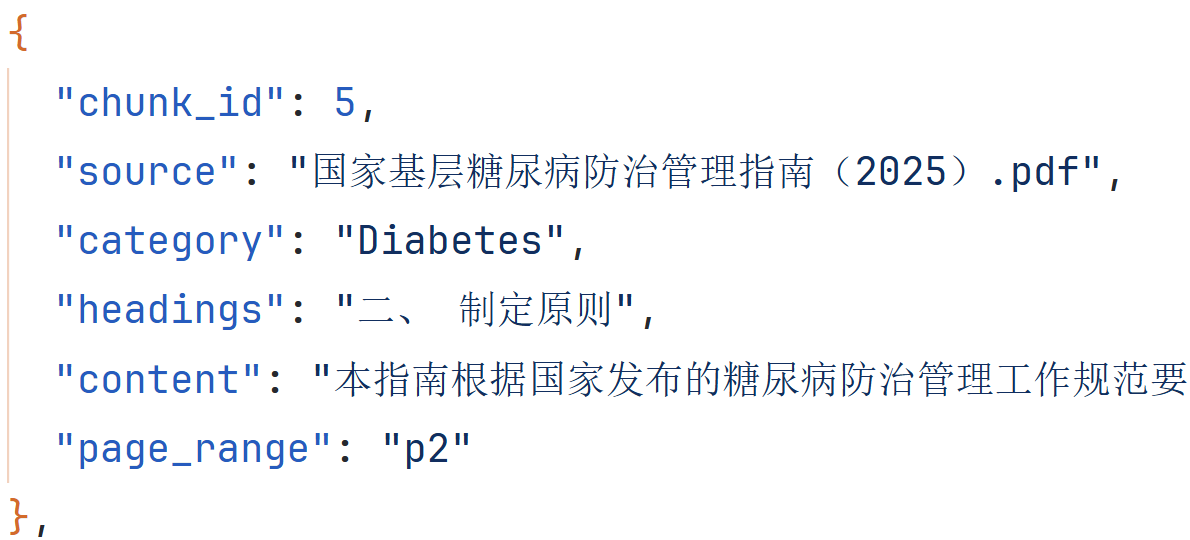
\includegraphics[width=0.7 \textwidth]{image/3/chunk.png}
    \caption{切分后的chunk示例}
    \label{fig:chunk}
\end{figure}

\subsection{Embedding向量化表示}

文本切分完成之后，知识库里的每个文本块都还需要经过一步转换，变成能够支持语义检索的向量表示。Embedding模型会把离散文本映射到一个统一的高维语义空间中，使语义相近的文本在向量空间中的距离更近，从而支持后续基于相似度的向量检索。

本系统采用BGE系列Embedding模型对医学文本块进行向量化处理。BGE模型具有较好的中文语义表示能力，能够较好地适应医学问答场景中常见的疾病名称、症状描述、用药建议以及生活化表达等多种文本形式。在知识库构建阶段，系统使用BGE模型对切分后的chunk逐条编码，生成对应的稠密向量；在在线检索阶段，则对用户问题执行相同的编码操作，并通过计算问题向量与知识块向量之间的相似度来完成召回。

Embedding向量化的意义在于，它把知识库的检索方式从单一依赖关键词匹配，转变成了兼具基于语义理解进行检索的能力；针对医学问答中大量存在的同义表达、口语化描述和隐含问题，这种向量化表示正是扩大召回覆盖面、增强检索稳健性的关键基础。

\subsection{向量数据库构建}

在获得文本块的向量表示后，还需要构建能够支持高效近邻检索的向量数据库或向量索引结构。若仅对全部向量进行线性遍历比对，在知识规模增长后会显著增加检索开销，难以满足在线问答场景对响应速度的要求。因此，知识库构建不仅包括文本组织和向量生成，也包括向量检索结构的建立。

本系统采用FAISS构建医学知识库的向量索引，把每个文本块向量与它对应的原文内容、标题路径和来源信息建立起映射关系，这样在向量检索时系统既能快速获得与查询最相近的文本块，又能把结果回溯到原始文本内容和来源元数据，为后续的证据展示与可解释性分析提供支撑。

\section{医学文本检索方法}

\subsection{BM25关键词检索原理}

BM25是一种比较经典的关键词检索模型，主要根据查询词在文档中的出现情况来计算相关性，因此更适合处理以词面匹配为主的检索任务。对于查询$q$和文档$d$，它的得分公式可以写作
\begin{equation}
\mathrm{score}(q,d)=\sum_{t\in q}\mathrm{idf}(t)\cdot
\frac{f(t,d)\cdot(k_1+1)}{f(t,d)+k_1\cdot(1-b+b\cdot\frac{|d|}{\mathrm{avgdl}})}
\end{equation}
式中，$f(t,d)$表示词项$t$在文档$d$中的出现次数，$\mathrm{idf}(t)$表示逆文档频率，$|d|$表示文档长度，$\mathrm{avgdl}$表示平均文档长度，$k_1$和$b$则用来控制词频影响和长度归一化程度。

在医学问答场景里，疾病名称、药物名称、检查指标和各类专业术语往往具有很强的区分作用，而BM25正好比较擅长保留这类关键词信息，所以在精确匹配方面表现比较稳定。它的不足也很明显，就是对同义表达、口语化提问和更深一层的语义关系不够敏感，因此只依赖BM25时，系统容易漏掉一些意思接近但表述不同的内容。

\subsection{向量检索原理}

向量检索的思路和关键词检索不同，它不是直接看词是否匹配，而是先借助嵌入模型把用户问题和文档内容都表示成向量，再放到同一个语义空间中进行比较，语义越接近，向量之间通常也越接近，系统就更容易把对应文本检索出来。本文选用BGE-M3作为嵌入模型\cite{chen2025m3embeddingmultilingualitymultifunctionalitymultigranularity}，并把知识库中的每个文本块编码成稠密向量，再写入FAISS索引中保存。

在相似度计算方面，常见方法主要有余弦相似度和内积两种形式，当向量完成归一化以后，这两种做法在效果上可以看作基本一致。结合工程实现需求，本文在FAISS中采用内积检索方式，也就是IndexFlatIP，这样既能保持较高的检索效率，也能较好反映语义层面的接近程度。

和关键词检索相比，向量检索更擅长处理同义表达、上下位概念以及长句语义理解这类问题，比如提问方式发生变化以后，它仍然有可能找到意思接近的文本。不过，它对局部关键词的约束相对较弱，有时会召回语义上看起来相关、但关键实体并不一致的文本片段。医学问答对术语准确性要求较高，所以只依靠向量检索也很难保证结果始终稳定，通常还需要和关键词检索配合使用。

\subsection{混合检索策略}

为兼顾“术语精确匹配”与“语义泛化召回”两个目标，本文采用BM25与向量检索的混合策略，并设计了一条“双路召回到融合排序再到重排精筛”的处理流程：

第一步，系统让两种检索逻辑各自独立地从知识库中检索出各自认为最相关的候选文档列表，形成两路结果；第二步，对这双路结果执行融合排序，采用的算法是倒数排序融合，它的计算形式可以写作：

\begin{equation}
RRF(d)=\sum_{r\in R}\frac{1}{k+r(d)}
\end{equation}
其中R代表参与融合的各路排序列表的集合，r(d)表示某篇文档d在对应列表中的排列位次，k是一个用来平滑结果的常数，本系统取k=60，这个公式综合了一篇文档在不同排序列表中的名次信息，名次越靠前最终得分越高；第三步，融合出统一的候选列表后，再引入BGE-Reranker-v2-M3的专门重排模型，对候选文档进行交叉编码式的高精度重排，最终截取出靠前的Top-K份证据。

与单用一种检索方式相比，混合策略有几方面的好处：第一，BM25防止了关键专业术语不会因为语义而无法被准确检索；第二，向量检索弥补了同义改写和口语表达的语义召回盲区；第三，重排模型进一步提升了最终送去给生成模型用的证据的相关性，有效滤掉那些“初看沾边但不支持直接做答”的噪声片段；这样的组合策略，在同一套检索链路里同时回应了医学问答对“高召回”和“高精度”的双重严苛要求。

\section{实验与结果分析}

为了验证不同检索方法在医学知识库中的实际召回效果，本文围绕已经构建完成的FAISS索引开展了检索实验。实验中，先从知识库里随机抽取60个文本段，再根据这些文本段的内容人工设计相关问题，每个问题都对应一个预期命中的目标文本块，只要这个目标文本块出现在前$K$个检索结果中，就记作一次命中。本文选用Recall@1、Recall@5和Recall@10作为评价指标，用来衡量系统在只返回1条、前5条和前10条候选结果时的召回能力。

实验共比较了三种检索方式，一种是基于BM25的关键词检索，一种是基于BGE向量表示和FAISS索引的向量检索，另一种是本文采用的混合检索策略，也就是先结合BM25和向量检索进行双路召回，再通过Reranker完成重排，最后给出排序结果。三种方法的实验结果如表\ref{tab:rag-recall-results}所示。

\begin{table}[htbp]
    \caption[RAG检索方法Recall@$K$对比结果]{RAG检索方法Recall@$K$对比结果}
    \centering
    \begin{tabular}{lccc}
        \toprule
        检索方法 & Recall@1 & Recall@5 & Recall@10 \\
        \midrule
        BM25检索 & 0.26 & 0.81 & 0.92 \\
        向量检索 & 0.48 & 0.81 & 0.85 \\
        混合检索 + Rerank重排 & 0.59 & 0.89 & 0.96 \\
        \bottomrule
    \end{tabular}
    \label{tab:rag-recall-results}
\end{table}

从实验结果来看，三种检索方法在不同$K$值下表现出比较明显的差异。先看Recall@1，BM25检索为0.26，说明如果系统只返回首条结果，只依靠关键词匹配很难稳定命中目标文本；向量检索的Recall@1提升到0.48，说明语义检索对口语化表达、近义改写和不完全词面匹配的问题有更好的适应能力；混合检索结合Rerank重排以后，Recall@1进一步提升到0.59，是三种方法中最高的。这说明在最靠前的排序位置上，混合检索策略更容易把真正相关的证据提前放出来。

再看Recall@5，BM25检索和向量检索都达到0.81，混合检索则提升到0.89。这说明当候选范围扩大到前5条时，单一检索方法已经能够召回大部分相关文本，但仍然会出现一定程度的漏召回；相比之下，混合检索同时利用了关键词匹配和语义匹配两类信息，又经过重排模型进一步筛选，因此在前5条结果里保留了更多有效证据。对RAG系统来说，这一点很重要，因为生成模型通常不会使用过多检索结果，如果前几条证据质量不够高，最终回答质量也会直接受到影响。

最后看Recall@10，BM25检索达到0.92，高于向量检索的0.85，这说明当候选集合进一步放宽以后，BM25在专业术语、数字指标这类关键词层面的覆盖能力会更明显，更容易把目标文本放进较长的候选列表里。不过，混合检索加Rerank重排的Recall@10仍然达到0.96，依然是三种方法中最好的结果。这说明混合检索并不是简单把两种方法拼在一起，而是在不同检索机制之间形成了比较明显的互补关系，BM25负责尽量保住专业术语、药物名称和指标数值这类关键信息不被漏掉，向量检索负责补足语义层面的相似表达，重排模型再进一步减少“看起来相关、但并不是最佳证据”的干扰。

综合来看，单独使用BM25更适合术语比较明确的问题，但对自然语言表达变化会更敏感；单独使用向量检索在语义匹配上更有优势，不过在一些依赖精确术语和细粒度实体区分的问题上，仍然可能出现误召回。相比之下，混合检索结合重排策略在Recall@1、Recall@5和Recall@10三个指标上都取得了最好结果，说明这种方法更适合医学问答场景中“专业术语精确匹配”和“自然语言语义召回”同时存在的需求。因此，本文最终选择混合检索加Rerank重排作为RAG问答系统的默认检索方案。

\section{本章小结}

本章前半部分围绕医学知识库构建与检索方法展开，介绍了知识数据来源、文本预处理、语义切分、Embedding向量化表示以及向量索引构建过程，并进一步分析了BM25、向量检索和混合检索策略在医学问答场景中的特点与差异。实验结果表明，混合检索结合重排策略在召回覆盖和结果稳定性方面表现更好，能够为后续回答生成提供更可靠的证据基础。

通过这一部分的研究，系统已经基本解决了“回答依据从哪里来”的问题，也为后续围绕RAG输入组织、Prompt设计和模型优化展开分析提供了支撑。

\chapter{系统设计与实现}

\section{系统设计目标}

针对“三高”慢性病医学问答场景中专业信息较多、回答可靠性要求较高、交互反馈也比较明显的特点，本文设计并实现了一套基于检索增强生成的智能医学问答系统，并结合医学问答任务本身的需求，提出了四个方面的系统设计目标。

一是准确性，医学问答系统首先要尽量保证回答内容科学、准确，因为医学知识本身专业性很强，一旦出现错误或表述不严谨，就可能误导用户，甚至带来潜在风险。为了解决这个问题，系统构建了较高质量的“三高”慢性病医学知识库，并采用关键词检索和语义向量检索结合的混合检索策略，从权威资料中找出和用户问题高度相关的医学证据，再借助RAG机制把这些证据送入大语言模型作为回答依据，从而减少模型凭空编造内容的情况，提高回答的事实一致性和专业可靠性。

二是可解释性，和通用问答系统相比，医学问答不只是给出结论，还要让使用者看清结论依据来自哪里。基于这一点，系统在生成回答时，会同时保留并展示相关医学证据的来源信息，比如指南、科普文章或其他参考资料，通过“回答正文加引用来源”的形式，让结论来源能够被进一步追溯；同时，系统也会在提示词设计中对模型输出加入结构化约束，引导生成内容尽量围绕检索到的证据展开，从而进一步增强结果的可解释性。

三是实时性，在实际使用过程中，用户通常希望较快得到问答结果，因此系统需要具备较好的响应速度。考虑到大语言模型推理本身计算开销较大，系统将模型部署在高性能服务器上，并加入多种性能优化方式，包括利用向量检索加快知识匹配过程、使用混合精度计算降低推理开销，以及通过键值缓存减少重复计算，从而提升整体生成效率；在系统架构上，系统还采用前后端分离设计，使用户请求能够更快完成处理和返回，以满足实时交互的需要。

四是可扩展性，医学知识会不断更新，应用需求也会持续变化，因此系统还需要保留较好的扩展能力。一方面，知识库采用模块化管理方式，支持医学数据的新增、修改和维护，便于后续持续纳入新的医学指南和研究成果；另一方面，系统在架构设计上让知识库、检索模块和生成模型之间保持相对松耦合的关系，使各部分能够独立升级或替换，比如可以在不影响整体结构的情况下更换性能更好的向量模型或大语言模型，这样也能为系统后续的演进和适应能力留出足够空间。

\section{系统总体架构}

本系统整体架构采用分层式设计，将交互逻辑、业务逻辑、模型能力与数据能力进行划分，各模块之间相对独立，能够在一定程度上实现故障隔离。系统架构如图4.1所示，主要由四个层次构成。

前端应用层只承担交互和状态管理，不直接参与模型推理，具体包括用户登录、会话管理、消息渲染、流式展示、引用证据呈现以及管理员知识库入口等功能。

业务服务层基于Node.js，采用Express框架构建统一的 API 网关，用于对外提供服务接口。业务服务层主要负责身份认证与权限控制、会话上下文组织、消息持久化、模型服务编排和知识库维护。

模型推理层是一套独立的Python服务，部署在高性能GPU服务器上，基于Flask框架对外提供接口。该层主要负责向量数据库检索、相关文档重排序、提示词组装、模型推理及流式事件输出。模型服务对外暴露同步与流式两类接口，业务服务可以根据实际场景灵活选择调用方式。将推理服务独立部署后，可在不影响业务API的情况下单独升级模型和检索策略。

数据与索引层中使用关系型数据库保存用户、会话、消息与文档元数据；使用FAISS向量索引存储医学指南等医学资料，并将文本编码为向量构建索引结构以支持向量检索和BM25检索。

\vspace{10pt}
\begin{figure}[htb]
    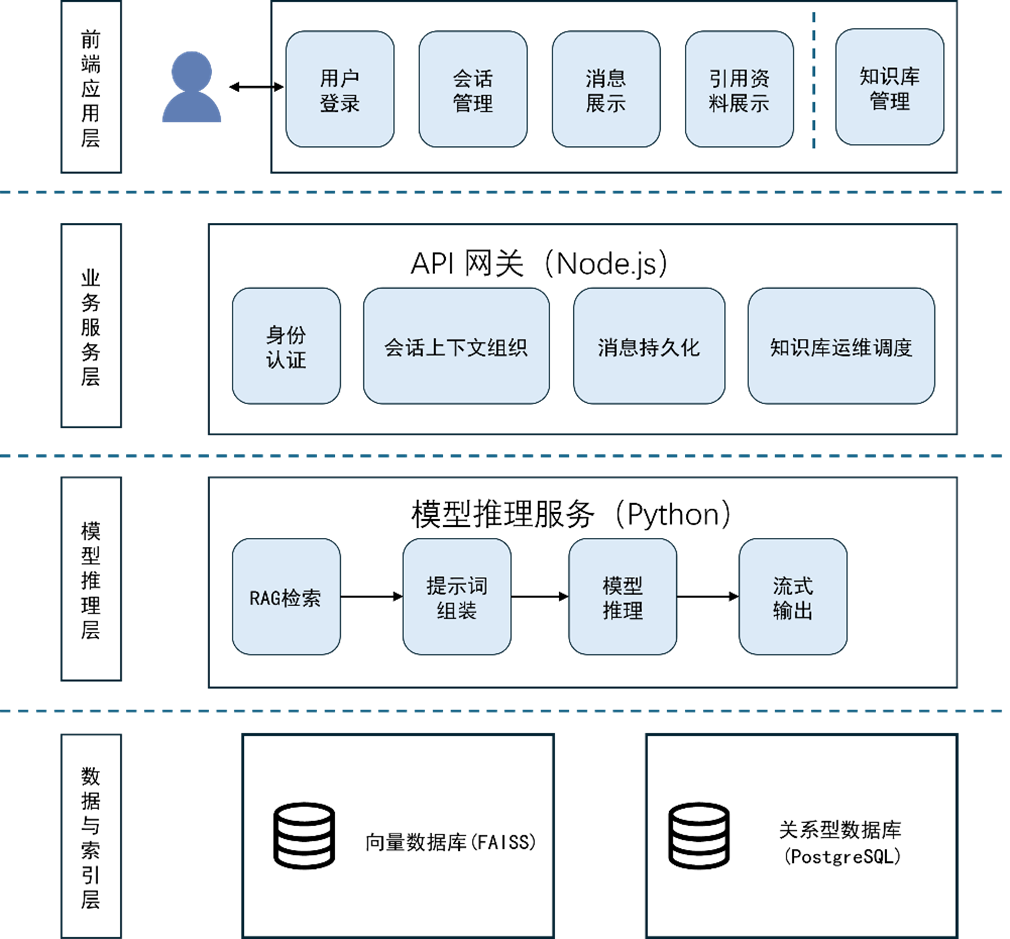
\includegraphics[width=0.7 \textwidth]{image/4/系统架构图.png}
    \caption{系统架构图}
    \label{fig:framework-structure}
\end{figure}

\section{系统流程设计}

在输入解析阶段，系统会先接收用户发来的自然语言问句，再结合之前几轮对话的历史信息对查询做语义补全和规范化处理，从而让后续检索能更精准地锁定用户真正的意图。

在知识检索阶段，系统采用混合检索策略，一路是基于向量的语义检索，它依靠Embedding模型把文本映射到高维的向量空间中来表示语义、捕捉深层的语义相似性；另一路则是基于关键词的BM25检索，专门负责精确锁定关键字上的匹配，特别针对于医学领域海量的专业术语。如果只依赖向量检索，有可能会漏掉或误判某些关键医学名词，于是把BM25作为补充手段能有效提高整个检索结果的准确度和覆盖面，两路结果检索完成之后，系统再经过融合、排序和重排这几道处理，筛选出最相关的一批文本片段。

在上下文增强阶段，系统将上一阶段筛选出的文本片段，用户问题和对话历史，通过事先设计好的prompt模板结合，构建成一份结构清晰的输入，让模型在阅读时能轻易分辨出哪一部分来自使用者的提问、哪一部分是从知识库里调出来的参考资料。

在答案生成阶段，模型依据这份组合好的输入来产出回答，以流式方式逐字输出。在生成全部完成后，系统会把检索到的文献信息返还给用户当成参考，同时也会记录下这次输入和输出所消耗的token数量，后者将会跟对话历史一同保存进数据库，为下一次用户提问时构建多轮对话上下文时估算长度提供依据。

\section{业务层实现}

业务层后端服务基于Node.js的框架Express开发，负责用户身份认证与权限控制、会话管理、消息持久化、模型服务编排与知识库运维接口。

\subsection{后端服务架构设计}

系统后端入口位于统一应用服务中，主要路由模块包括用户认证、会话管理、消息管理、模型调用和知识库管理。各模块职责如下：
\begin{enumerate}[label =(\arabic*)]

    \item 认证模块：提供注册与登录接口，完成密码加密与令牌签发；
    \item 会话模块：管理会话创建、查询、更新与软删除；
    \item 消息模块：管理消息读写与 token 信息回填；
    \item 模型模块：接收问题请求，调用本地模型服务并返回生成结果；
    \item 知识库模块：提供文档元信息管理、索引状态查询与重建能力。

\end{enumerate}

\subsection{会话管理}

会话管理是后端业务逻辑中的核心部分。系统为每个用户维护独立会话空间，并将每轮对话中的角色、正文、时间戳、引用证据和统计信息写入数据库，以支撑历史记录查询和多轮上下文组织。

在具体流程上，当用户提交问题时，后端会先判断当前会话是否存在；若不存在，则创建新会话并写入用户消息；若已存在，则直接在原会话下追加消息。模型返回回答后，系统再将助手回答与证据一并写回，并同步更新会话摘要和更新时间。这样既能保证多轮对话连续性，也方便前端展示最近会话状态。

\subsection{数据库}

后端数据库使用PostgreSQL，PostgreSQL可支持使用“JSONB内容字段”的存储。在保存用户与模型的对话历史时，用户消息和模型消息、系统消息的结构并不完全相同，例如：模型消息在返回时会携带RAG过程中检索到的资料信息，而用户消息则不需要这个字段。面对这类字段需求参差不齐的情况，JSONB 格式比常规的关系型表设计要灵活得多，能很好地应对问答消息里字段不固定、结构可能时常变动的状况。系统将用户、会话、消息等较为固定的实体信息保存在关系型字段里；将消息正文、引用资料信息、Token消耗等可选字段的内容存放在JSONB字段中。通过这一混合存储方式，就能用同一张表适应模型消息和用户消息的不同格式，不必再去为每一种消息单独建表。 

表4.1中列出了系统中关键的数据表及其主要字段，其中，users表用于存储用户信息，并且为每个用户分配独特的id，用户id是对其他表查询的关键信息；conversations表用于存储会话元信息（标题、更新时间、软删除标记等）；messages表用于保存逐轮对话内容与token统计信息；medical\_documents表用于保存知识文档元数据；knowledge\_index\_meta表用于记录索引状态（dirty/running/synced/error）。

\begin{table}[htbp]
    \centering
    \caption{后端核心数据表}
    
    \setlength{\tabcolsep}{8pt} % 列间距（原来14mm太大了）
    
    \begin{tabular}{l c p{5cm}} % 第三列自动换行
        \toprule
        数据表名 & 核心字段 & 作用 \\
        \midrule
        user & id, password\_hash, is\_admin & 用户身份与权限管理 \\
        conversations & user\_id, title, last\_message, is\_deleted & 会话元信息管理 \\
        messages & conversation\_id, role, content, tokens & 多轮消息与 token 信息存储 \\
        medical\_documents  &  title, source, ingest\_key, tags &  知识文档元信息维护 \\
        knowledge\_index\_meta  &  status, last\_reindexed\_at, last\_error  &  索引状态追踪与运维监控 \\
        \bottomrule
    \end{tabular}
\end{table}

\subsection{流式转发}

为了缩短用户等待时的空白感，后端加入了面向前端的流式转发机制，Node.js服务接收到模型服务返回的增量文本后，会继续通过SSE把内容持续发送到前端，这样回答还没有完全生成时，界面上就已经能看到文本逐步显示出来，整体交互会更连贯。

具体处理时，后端会先把用户消息和助手占位消息写入数据库，再和模型服务建立流式连接，后续只要模型服务持续返回新的文本片段，后端就会把这些内容整理成前端可以解析的事件数据并立即转发出去；等回答生成结束后，再统一回写完整结果和相关统计信息，这样一来，界面能够及时更新，数据库里保存的内容也能保持完整一致。

\subsection{知识库管理接口}

知识库管理接口主要面向管理员使用，任务是把文档维护和索引管理这一类后台操作组织起来，接口内容包括文档元信息查询、文本上传入库、索引状态查看、增量更新和全量重建等，这样知识库相关操作就能放在统一入口中处理，管理起来也更方便。

在知识入库过程中，后端接收到文本内容和来源信息后，会继续调用后续处理流程，依次完成文本清洗、内容切分、Embedding编码和索引写入，写入成功以后，再触发模型服务对索引进行热更新；如果中间某个环节出现问题，系统会把错误状态记录下来，并返回较明确的提示信息，方便后面排查和恢复，这样处理之后，知识更新就不再是彼此分散的单独步骤，而是能和在线问答过程更自然地衔接起来。

\section{模型服务实现}

\subsection{Qwen推理服务}

模型服务采用Python独立实现，其中Qwen推理模块负责最终回答生成。系统启动时加载基础模型和分词器，并根据资源条件选择相应推理方式。问答过程中，模型服务接收后端转发的问题、上下文和参数配置，将其组织为统一输入后交给Qwen模型执行生成。

选择Qwen作为生成核心，主要考虑其中文能力较强，且能够较好处理长上下文和说明性回答。与RAG和DPO模块结合后，Qwen不仅承担“生成文本”的任务，也成为系统将检索证据转化为自然语言答复的关键执行单元。

\subsection{bge Embedding服务}

为支持语义检索，模型服务内部集成bge Embedding模型，对用户查询和知识文本进行向量化表示。知识入库阶段，系统对文本块编码并写入向量索引；在线问答阶段，再对用户问题执行同样的编码操作，以完成相似度检索。

Embedding服务的价值在于，它让系统能够理解不同表述之间的语义接近关系，而不必拘泥于字面一致。对于大量口语化、症状化的慢病咨询问题，这一点尤为重要。

\subsection{DPO模型加载与推理}

除基础Qwen模型外，系统还支持加载经DPO训练得到的适配权重，以进一步优化医学场景下的回答偏好。部署时，这部分权重通常以适配器形式保存，模型服务按配置完成加载，并与基础模型共同组成最终推理模型。

在实际推理中，DPO优化不会改变检索结果本身，但会影响模型如何组织回答。例如，当问题涉及治疗建议、用药风险或证据不足时，模型会更倾向于采用审慎表述，并主动提醒线下就医或补充信息。这种变化正是偏好优化在医学场景中的主要价值。

\subsection{流式输出}

模型服务同时支持同步生成和流式生成两种模式。流式模式下，服务会持续返回模型生成的文本片段，使回答具备边生成边展示的效果，从而明显改善交互体验。

在实现上，模型服务通过SSE事件格式向后端发送\texttt{delta}、\texttt{end}和\texttt{error}等事件；后端再将这些事件继续转发到前端，形成端到端的流式问答链路。这一设计让系统既能保持低时延反馈，也能在异常情况下提供较清晰的错误处理路径。

\section{RAG服务工程实现}

\subsection{检索调用流程}

在RAG服务运行时，模型服务首先接收用户问题，并结合必要的历史对话构造检索查询。随后，系统并行调用BM25和向量检索，分别得到关键词相关候选和语义相关候选，形成双路初召回结果。

完成召回后，系统对候选文本进行统一标识、合并与去重，再进入融合排序和重排阶段。最终保留下来的高质量证据会被组织为结构化上下文，并传递给生成模块。整个流程强调的是“先保证不漏，再尽量选准”。

\subsection{BM25 + 向量融合实现}

在工程实现上，BM25和向量检索保持相对独立的召回路径，系统在候选层面对两类结果进行统一融合。BM25负责抓住关键术语，向量检索负责补足语义改写，两者组合后能够更稳妥地应对真实问答中的表达差异。

融合时，系统根据候选在不同检索列表中的相对位置综合计算优先级，使在多路检索中都表现靠前的文本获得更高排序。这样做避免了单一路径偏差对最终结果造成过大影响。

\subsection{Rerank实现}

融合后的候选结果仍可能包含主题相关但并不适合直接作答的文本，因此系统进一步引入重排模型进行精筛。与初召回不同，重排阶段更关注“这段文本是否最适合回答当前问题”，而不是“它是否大致相关”。

在实现中，系统逐条计算候选证据与问题之间的匹配程度，并据此重新排序，再从中选出Top-$K$文本作为最终证据。该步骤能够明显降低噪声片段进入生成阶段的概率，是提升回答质量的重要环节。

\subsection{上下文拼接}

在获得最终证据后，系统需要将其组织成模型可直接利用的输入上下文。拼接时，系统会保留证据来源、标题和正文片段，并按相关性顺序写入Prompt中，使模型既能看到内容本身，也能感知其来源背景。

同时，系统会控制证据条数和单条长度，避免长文本挤占过多上下文空间。对于多轮问答，还会加入必要的近期历史消息，以帮助模型更准确地理解当前问题与前文之间的关系。

\section{前端实现}

\subsection{前端UI架构与路由设计}

前端界面采用React构建，并结合路由机制完成页面切换，整体上分为登录页、注册页、问答主页和知识库管理页，不同页面各自承担明确任务，这样既方便功能拆分，也有利于后续继续补充新模块。登录和注册页面主要处理身份验证，问答主页负责会话列表、消息展示和问题输入，知识库管理页则面向管理员，用来处理文档维护与索引相关操作。

在界面组织上，前端把通用能力拆分到页面、组件和Hook三个层次，页面负责整体布局和功能组合，组件负责消息列表、输入框、侧边栏等可复用界面，Hook负责会话状态、消息请求和交互流程管理，这种划分方式能让界面结构更清楚，代码之间的联系也更容易梳理。主页部分采用侧边栏与主内容区的布局，侧边栏用于展示历史会话和常用操作，主区域用于展示问答内容与输入区域，页面层次比较直观，用户进入系统后也能较快找到对应功能。

\subsection{对话交互与流式渲染实现}

会话相关的核心逻辑集中放在自定义Hook中，发送问题时，界面会先把用户消息和助手的占位内容加入当前会话，再向后端发起流式请求，这样用户提交问题后能马上看到界面变化，等待过程也不会显得突兀。流式数据通过后端的SSE通道持续返回，前端再用ReadableStream按帧读取并解析事件，接收到\texttt{delta}内容后，就把新增文本接到助手回答后面，于是回答会一点点展开，形成较自然的实时反馈效果。

为了让多轮对话前后保持一致，流式输出结束后，前端还会重新拉取一次消息记录，并用后端已经保存的结果覆盖临时状态，避免在长对话过程中因为局部丢帧或上下文偏移，出现界面显示和实际数据不一致的情况；如果模型服务中途异常或连接中断，界面会直接给出明确的提示文本，使当前交互还能继续恢复，不会停在难以理解的状态里。

\subsection{消息展示与检索证据可视化}

消息展示部分支持Markdown和GFM语法渲染，因此回答中的分点说明、表格以及部分结构化内容都能较完整地显示出来，页面阅读体验也更清楚。在RAG问答场景下，系统会把检索得到的\texttt{retrieved\_docs}附加到助手消息中，再在回答下方用“全部引用”的折叠区域统一展示，这样答案和证据能够放在同一界面里，用户查看结论时也能顺带看到对应依据，有助于增强结果的可解释性与可追溯性。

为了减少重复信息，前端会按照\texttt{source}字段对引用文档进行去重，同时保留来源名称、标题层级等关键内容，便于快速核对回答依据，也便于进一步判断相关结论是否来自较可靠的医学资料，从而提高对系统输出结果的信任程度。

\section{本章小结}

本章从工程实现角度介绍了医学问答系统的整体设计。首先明确了系统在准确性、可解释性、实时性和可扩展性方面的目标；随后说明了总体架构和RAG运行流程；最后分别从后端、模型服务、RAG工程实现和前端交互四个层面展开具体实现分析。

通过上述设计与实现，本文完成了一套具备知识检索、模型生成、证据展示和会话管理能力的医学问答系统，为后续实验评估和应用验证提供了完整工程基础。

\chapter{系统设计与实现}

\section{系统设计目标}

针对“三高”慢性病医学问答场景中信息专业性强、回答可靠性要求高以及实时交互需求明显的特点，本文设计并实现了一种基于检索增强生成的智能医学问答系统，在综合分析医学问答任务特点的基础上，设定了四个方面的设计目标。

第一个方面是准确性，医学问答系统首先要保证回答内容的科学性与准确性，因为医学知识具有高度专业性，错误或不严谨的信息可能对用户产生误导甚至带来潜在风险，为了应对这一问题，本系统构建了高质量的“三高”慢性病医学知识库，并采取关键词检索与语义向量检索相结合的混合检索策略，从权威资料中获取与用户问题高度相关的医学证据，再引入RAG机制，把检索到的证据作为约束条件输给大语言模型，从而有效抑制模型自行编造内容的幻觉现象，提升回答的事实一致性与专业可靠性。

第二个方面是可解释性，与通用问答系统不同，医学问答不仅需要给出结论，还要让用户能够理解答案的依据来源，为此本系统在生成回答的同时保留并展示相关的医学证据来源信息，比如指南或科普文章，通过展示“回答正文加上引用来源”的结构让用户能够追溯信息源头，同时在提示语设计中对模型输出施加结构化约束，促使生成内容尽可能围绕检索到的证据展开，进一步增强系统的可解释性。

第三个方面是实时性，在实际应用场景里用户通常期望快速获得问答结果，这就要求系统具备良好的响应速度，考虑到大语言模型推理的计算开销较大，本系统把大语言模型部署在高性能服务器上并引入多种性能优化策略，包括用向量检索来加速知识匹配过程、利用混合精度计算降低模型推理开销、以及通过键值缓存机制减少重复运算，从而显著提升生成效率，同时在系统架构层面采用前后端分离设计，使用户请求能被快速处理并返回结果，满足实时交互的需求。

第四个方面是可扩展性，随着医学知识的持续更新和应用需求的不断拓展，系统需要具备良好的扩展能力，一方面知识库设计采用模块化管理方式，支持医学数据的增删操作，便于持续纳入新的医学指南和研究成果，另一方面在系统架构上把知识库、检索模块与生成模型彼此之间保持松耦合关系，使各模块能独立升级或替换，比如可以在不影响整体系统结构的情况下更换更高性能的向量模型或大语言模型，从而保证系统在未来具备良好的演进能力与适应性。

\section{系统总体架构}

本系统整体架构采用分层式设计，将交互逻辑、业务逻辑、模型能力与数据能力进行划分，各模块之间相对独立，能够在一定程度上实现故障隔离。系统架构如图\ref{fig:framework-structure}所示，主要由四个层次构成。

前端应用层只承担交互和状态管理，不直接参与模型推理，具体包括用户登录、会话管理、消息渲染、流式展示、引用证据呈现以及管理员知识库入口等功能。

业务服务层基于Node.js，采用Express框架构建统一的 API 网关，用于对外提供服务接口。业务服务层主要负责身份认证与权限控制、会话上下文组织、消息持久化、模型服务编排和知识库维护。

模型推理层是一套独立的Python服务，部署在高性能GPU服务器上，基于Flask框架对外提供接口。该层主要负责向量数据库检索、相关文档重排序、提示词组装、模型推理及流式事件输出。模型服务对外暴露同步与流式两类接口，业务服务可以根据实际场景灵活选择调用方式。将推理服务独立部署后，可在不影响业务API的情况下单独升级模型和检索策略。

数据与索引层中使用关系型数据库保存用户、会话、消息与文档元数据；使用FAISS向量索引存储医学指南等医学资料，并将文本编码为向量构建索引结构以支持向量检索和BM25检索。

\vspace{10pt}
\begin{figure}[htb]
    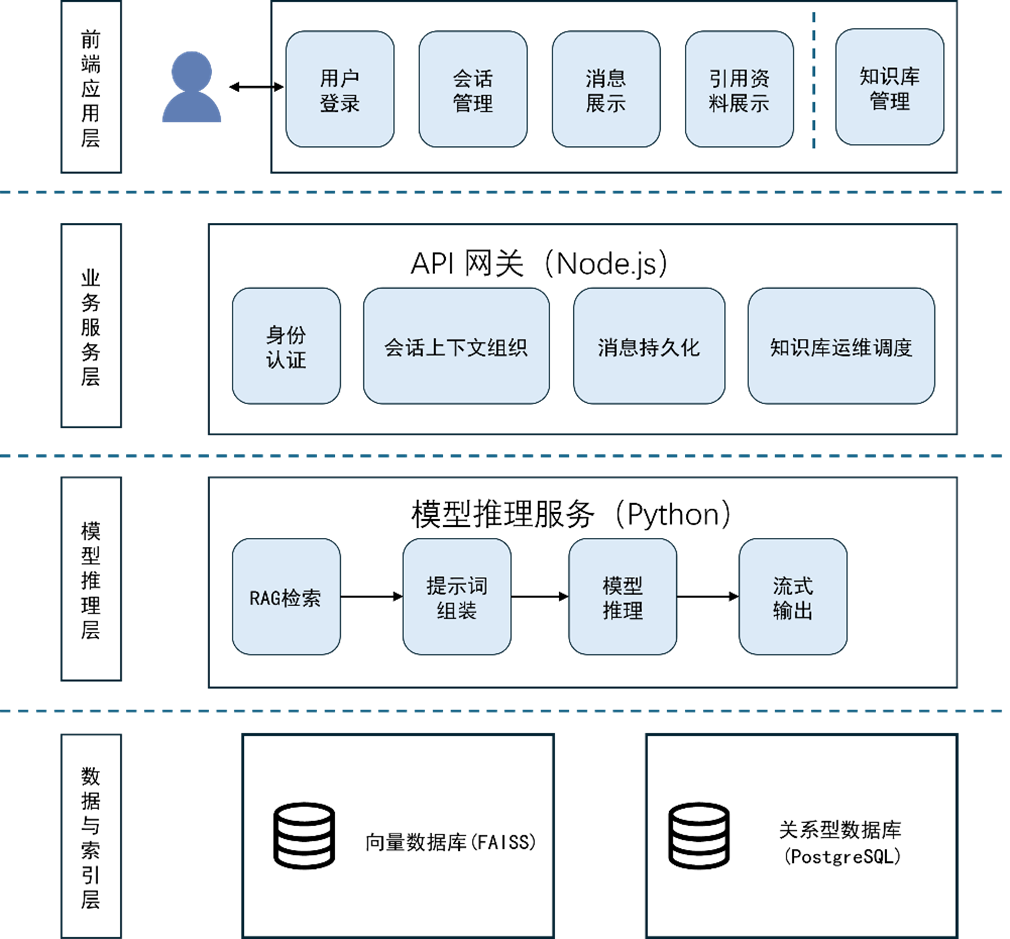
\includegraphics[width=0.8 \textwidth]{image/4/系统架构图.png}
    \caption{系统架构图}
    \label{fig:framework-structure}
\end{figure}

\section{系统流程设计}

针对“三高”慢病管理场景，本文将问答流程划分为“输入解析—知识检索—上下文增强—答案生成”四个阶段。系统流程如\ref{fig:system-flowchart}所示。

\vspace{10pt}
\begin{figure}[htb]
    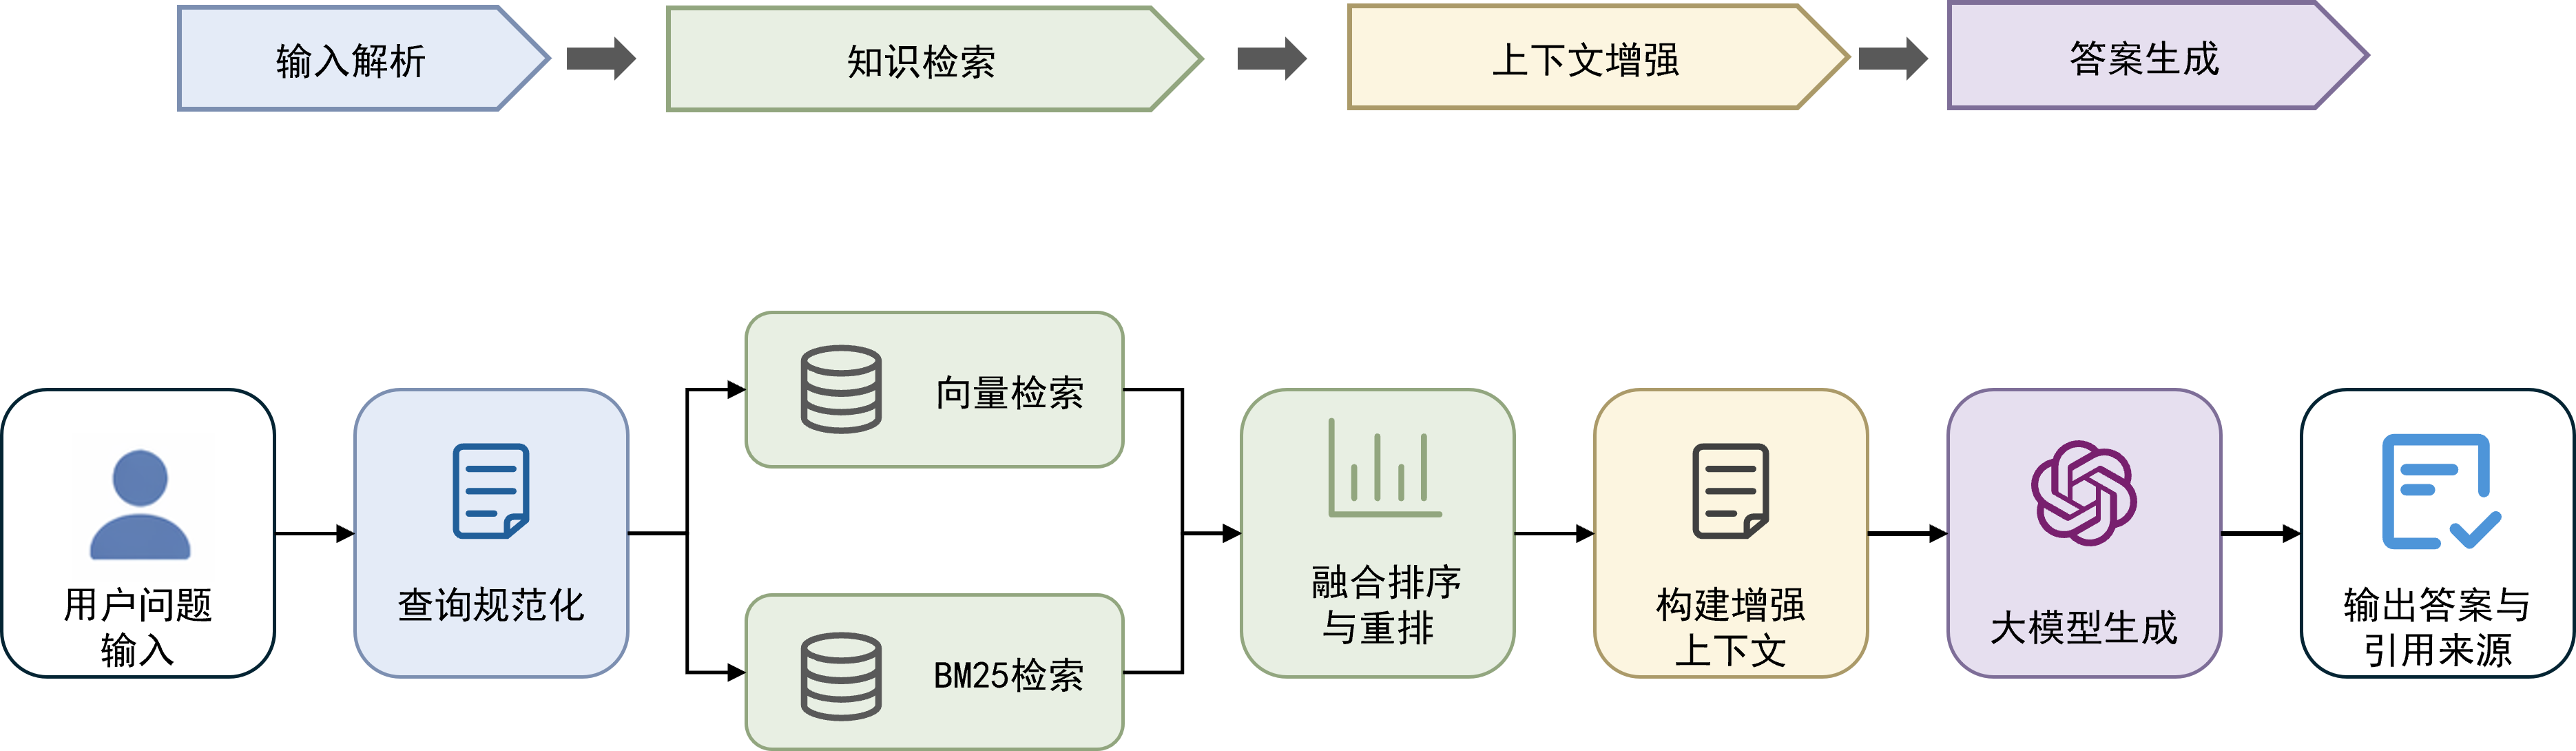
\includegraphics[width=0.8 \textwidth]{image/4/framework.png}
    \caption{系统流程图}
    \label{fig:system-flowchart}
\end{figure}

在输入解析阶段，系统会先接收用户发来的自然语言问句，再结合之前几轮对话的历史信息对查询做语义补全和规范化处理，从而让后续检索能更精准地锁定用户真正的意图。

在知识检索阶段，系统采用混合检索策略，一路是基于向量的语义检索，它依靠Embedding模型把文本映射到高维的向量空间中来表示语义、捕捉深层的语义相似性；另一路则是基于关键词的BM25检索，专门负责精确锁定关键字上的匹配，特别针对于医学领域海量的专业术语。如果只依赖向量检索，有可能会漏掉或误判某些关键医学名词，于是把BM25作为补充手段能有效提高整个检索结果的准确度和覆盖面，两路结果检索完成之后，系统再经过融合、排序和重排这几道处理，筛选出最相关的一批文本片段。

在上下文增强阶段，系统将上一阶段筛选出的文本片段，用户问题和对话历史，通过事先设计好的prompt模板结合，构建成一份结构清晰的输入，让模型在阅读时能轻易分辨出哪一部分来自使用者的提问、哪一部分是从知识库里调出来的参考资料。

在答案生成阶段，模型依据这份组合好的输入来产出回答，以流式方式逐字输出。在生成全部完成后，系统会把检索到的文献信息返还给用户当成参考，同时也会记录下这次输入和输出所消耗的token数量，后者将会跟对话历史一同保存进数据库，为下一次用户提问时构建多轮对话上下文时估算长度提供依据。

\section{业务层实现}

业务层后端服务基于Node.js的框架Express开发，负责用户身份认证与权限控制、会话管理、消息持久化、模型服务编排与知识库运维接口。

\subsection{后端服务架构设计}

系统后端入口位于统一应用服务中，主要路由模块包括用户认证、会话管理、消息管理、模型调用和知识库管理。各模块职责如下：
\begin{enumerate}[label =(\arabic*)]

    \item 认证模块：提供注册与登录接口，完成密码加密与令牌签发；
    \item 会话模块：管理会话创建、查询、更新与软删除；
    \item 消息模块：管理消息读写与 token 信息回填；
    \item 模型模块：接收问题请求，调用本地模型服务并返回生成结果；
    \item 知识库模块：提供文档元信息管理、索引状态查询与重建能力。

\end{enumerate}

\subsection{会话管理}

会话管理是后端业务逻辑中的核心部分。系统为每个用户维护独立会话空间，并将每轮对话中的角色、正文、时间戳、引用证据和统计信息写入数据库，以支撑历史记录查询和多轮上下文组织。

在具体流程上，当用户提交问题时，后端会先判断当前会话是否存在；若不存在，则创建新会话并写入用户消息；若已存在，则直接在原会话下追加消息。模型返回回答后，系统再将助手回答与证据一并写回，并同步更新会话摘要和更新时间。这样既能保证多轮对话连续性，也方便前端展示最近会话状态。

\subsection{数据库}

后端数据库使用PostgreSQL，PostgreSQL可支持使用“JSONB内容字段”的存储。在保存用户与模型的对话历史时，用户消息和模型消息、系统消息的结构并不完全相同，例如：模型消息在返回时会携带RAG过程中检索到的资料信息，而用户消息则不需要这个字段。面对这类字段需求参差不齐的情况，JSONB 格式比常规的关系型表设计要灵活得多，能很好地应对问答消息里字段不固定、结构可能时常变动的状况。系统将用户、会话、消息等较为固定的实体信息保存在关系型字段里；将消息正文、引用资料信息、Token消耗等可选字段的内容存放在JSONB字段中。通过这一混合存储方式，就能用同一张表适应模型消息和用户消息的不同格式，不必再去为每一种消息单独建表，或在一张表中留下大量的空字段。  

表\ref{tab:backend-core-tables}中列出了系统中关键的数据表及其主要字段，其中，users表用于存储用户信息，并且为每个用户分配独特的id，用户id是对其他表查询的关键信息；conversations表用于存储会话元信息（标题、更新时间、软删除标记等）；messages表用于保存逐轮对话内容与token统计信息；medical\_documents表用于保存知识文档元数据；knowledge\_index\_meta表用于记录索引状态（dirty/running/synced/error）。

\begin{table}[htbp]
    \centering
    \caption{后端核心数据表}
    
    \setlength{\tabcolsep}{8pt} % 列间距（原来14mm太大了）
    
    \begin{tabular}{l c p{5cm}} % 第三列自动换行
        \toprule
        数据表名 & 核心字段 & 作用 \\
        \midrule
        user & id, password\_hash, is\_admin & 用户身份与权限管理 \\
        conversations & user\_id, title, last\_message, is\_deleted & 会话元信息管理 \\
        messages & conversation\_id, role, content, tokens & 多轮消息与 token 信息存储 \\
        medical\_documents  &  title, source, ingest\_key, tags &  知识文档元信息维护 \\
        knowledge\_index\_meta  &  status, last\_reindexed\_at, last\_error  &  索引状态追踪与运维监控 \\
        \bottomrule
    \end{tabular}
    \label{tab:backend-core-tables}
\end{table}

\subsection{流式转发}

为了缩短用户等待时的空白感，后端加入了面向前端的流式转发机制，Node.js服务接收到模型服务返回的增量文本后，会继续通过SSE把内容持续发送到前端，这样回答还没有完全生成时，界面上就已经能看到文本逐步显示出来，整体交互会更连贯。

具体处理时，后端会先把用户消息和助手占位消息写入数据库，再和模型服务建立流式连接，后续只要模型服务持续返回新的文本片段，后端就会把这些内容整理成前端可以解析的事件数据并立即转发出去；等回答生成结束后，再统一回写完整结果和相关统计信息，这样一来，界面能够及时更新，数据库里保存的内容也能保持完整一致。

\subsection{知识库管理接口}

知识库管理接口主要面向管理员使用，任务是把文档维护和索引管理这一类后台操作组织起来，接口内容包括文档元信息查询、文本上传入库、索引状态查看、增量更新和全量重建等，这样知识库相关操作就能放在统一入口中处理，管理起来也更方便。

在知识入库过程中，后端接收到文本内容和来源信息后，会继续调用后续处理流程，依次完成文本清洗、内容切分、Embedding编码和索引写入，写入成功以后，再触发模型服务对索引进行热更新；如果中间某个环节出现问题，系统会把错误状态记录下来，并返回较明确的提示信息，方便后面排查和恢复，这样处理之后，知识更新就不再是彼此分散的单独步骤，而是能和在线问答过程更自然地衔接起来。

\section{模型与RAG服务实现}

\subsection{模型服务功能设计}

本文将模型推理部分独立部署为Python服务，并和业务后端解耦。这样设计有两点直接好处，一是可以把GPU资源集中用于检索和推理任务，减少和业务逻辑混合部署带来的资源竞争，二是后续即使替换Embedding模型、重排模型或生成模型版本，也不需要同步改动业务层接口。

在职责划分上，模型服务主要承担四类任务，一是接收业务层转发的问题、历史对话和生成参数，二是完成查询向量化、候选召回和重排，输出可供生成阶段使用的证据集合，三是按照提示词模板把问题、历史消息和检索证据组织成统一输入，再调用生成模型产出回答，四是以同步或流式方式把结果返回业务层，同时附带引用证据和必要状态信息。经过这样的拆分后，模型服务实际上成为系统中连接“知识检索”和“回答生成”的核心执行节点。

\subsection{模型加载与推理组织}

在具体实现中，模型服务启动后会预先加载Embedding模型、重排模型和生成模型，并在内存中保持可复用状态，减少重复初始化带来的时间开销。生成模型部分采用“基础模型 + 适配器权重”的组织方式，基础模型负责通用语言生成，DPO训练得到的适配器权重在加载后参与实际推理，用于改善医学场景下的回答风格、风险提示和边界控制能力。这种组织方式既保留了基础模型的通用表达能力，也便于后续持续迭代微调权重。

在推理流程上，模型服务不是接收问题后直接生成回答，而是按固定顺序执行“检索准备、候选筛选、上下文构建、模型生成”四个步骤。服务先根据用户问题构造检索查询，再调用检索与重排模块得到排序后的证据片段，随后把问题、历史消息和证据封装成模型输入，最后调用生成模型输出回答。通过这种流程化组织，模型服务能够把第4章提出的RAG方法和DPO优化能力稳定地落实到在线推理过程中。

\subsection{接口设计与结果返回}

为了适应不同交互场景，模型服务对外提供同步调用和流式调用两类接口。同步接口更适合调试、批量测试和非实时任务，调用方在一次请求中等待完整回答返回；流式接口更适合在线问答场景，模型服务会把回答拆成连续文本片段逐步输出，让前端能够边接收边展示，减少等待完整回答时的停顿感。

在返回内容上，模型服务不只输出最终回答文本，还会同时返回检索证据、引用来源和必要状态字段。对于流式模式，服务通过事件形式持续返回增量内容，并在结束时统一发送完成标记；如果推理过程中出现异常，则返回错误事件并附带错误信息，便于业务层捕获和提示。通过这种接口设计，模型服务向上对接业务后端时可以保持调用方式统一，向下也能兼容不同推理模式。

\subsection{RAG请求编排流程}

在线问答请求到达后，业务后端会先完成会话识别、历史消息提取和参数整理，再把当前问题、必要上下文和调用配置转发给模型服务。模型服务收到请求后，按预设顺序依次执行查询规范化、候选召回、结果筛选、上下文构造和回答生成，最后把完整结果回传给业务层。

这种编排方式的特点在于，RAG链路不是单一函数调用，而是一条由多个步骤组成的服务流程。每个步骤都有相对明确的输入和输出，例如召回阶段输出候选文本集合，重排阶段输出重新排序后的证据列表，上下文构建阶段输出可直接送入生成模型的结构化输入。通过这种分阶段组织，系统可以在不中断整体服务的前提下，对单个环节进行调试、替换和性能优化。

\subsection{检索链路调度}

在工程实现上，RAG服务通过统一调度入口管理检索相关步骤。系统不会把BM25检索、向量检索、融合排序和重排分别暴露为分散接口，而是由模型服务在内部完成链路编排，对外只表现为一次“检索增强问答”调用。这样设计可以减少业务层对底层检索细节的依赖，后续即使调整召回方式或更换重排模型，上层接口也不需要同步修改。

在调度过程中，系统先根据用户问题生成检索查询，再并行触发不同召回路径，随后对候选结果做统一编号、去重和排序。完成排序后，系统只保留数量受控的高相关证据进入下游生成流程，避免把大量低价值文本直接送入模型。也就是说，RAG服务在系统中的作用不只是“把资料找出来”，更重要的是在有限上下文窗口内尽可能选出最值得保留的证据。

\subsection{证据封装与结果回传}

完成检索和筛选后，RAG服务还需要把中间结果转换成适合业务层和前端使用的结构。为此，系统会把最终证据统一封装成结构化对象，其中包含文本内容、来源信息、标题路径、相关性顺序和必要标识字段。这样处理后，生成模型可以直接使用这些证据构造输入，业务后端也可以在回答完成后把同一份证据回写数据库，前端则能基于这些字段展示“引用来源”或“检索依据”等信息。

在结果返回阶段，RAG服务输出的不只是最终回答文本，还包括检索证据、引用元数据和必要状态字段。对系统来说，这一点很关键，因为医学问答不仅需要给出结论，还需要在工程上支持结果追溯。把检索证据和生成结果作为同一次调用的组成部分统一返回后，系统就能保持“回答内容”和“回答依据”之间的一致性。

\subsection{索引更新与一致性维护}

RAG服务的另一个关键实现点，是知识更新后的索引一致性维护。由于知识库内容不是静态不变的，系统在管理员新增、修改或删除文档后，需要重新执行文本切分、向量编码和索引写入等步骤。为了避免知识内容已经更新而检索结果仍停留在旧状态，系统在知识库管理接口和RAG服务之间建立了索引状态联动机制，当文档发生变化时，会同步更新索引状态标记，并在必要时触发增量更新或全量重建流程。

这样的设计使RAG服务不仅负责在线问答时的实时检索，也承担了知识检索能力持续可用的维护职责。只有索引状态、文档内容和在线服务三者保持一致，RAG系统才能在真实应用中稳定运行。因此，RAG服务工程实现的重点在于检索增强链路如何被稳定组织、如何与业务层协同、以及如何支持后续运维更新。

\section{前端实现}

\subsection{前端UI架构与路由设计}

前端界面采用React构建，并结合路由机制完成页面切换，整体上分为登录页、注册页、问答主页和知识库管理页，不同页面各自承担明确任务，这样既方便功能拆分，也有利于后续继续补充新模块。登录和注册页面主要处理身份验证，问答主页负责会话列表、消息展示和问题输入，知识库管理页则面向管理员，用来处理文档维护与索引相关操作。

在界面组织上，前端把通用能力拆分到页面、组件和Hook三个层次，页面负责整体布局和功能组合，组件负责消息列表、输入框、侧边栏等可复用界面，Hook负责会话状态、消息请求和交互流程管理，这种划分方式能让界面结构更清楚，代码之间的联系也更容易梳理。主页部分采用侧边栏与主内容区的布局，侧边栏用于展示历史会话和常用操作，主区域用于展示问答内容与输入区域，页面层次比较直观，用户进入系统后也能较快找到对应功能。

\subsection{对话交互与流式渲染实现}

会话相关的核心逻辑集中放在自定义Hook中，发送问题时，界面会先把用户消息和助手的占位内容加入当前会话，再向后端发起流式请求，这样用户提交问题后能马上看到界面变化，等待过程也不会显得突兀。流式数据通过后端的SSE通道持续返回，前端再用ReadableStream按帧读取并解析事件，接收到delta内容后，就把新增文本接到助手回答后面，于是回答会一点点展开，形成较自然的实时反馈效果。

为了让多轮对话前后保持一致，流式输出结束后，前端还会重新拉取一次消息记录，并用后端已经保存的结果覆盖临时状态，避免在长对话过程中因为局部丢帧或上下文偏移，出现界面显示和实际数据不一致的情况；如果模型服务中途异常或连接中断，界面会直接给出明确的提示文本，使当前交互还能继续恢复，不会停在难以理解的状态里。

\subsection{消息展示与检索证据可视化}

消息展示部分支持Markdown和GFM语法渲染，因此回答中的分点说明、表格以及部分结构化内容都能较完整地显示出来，页面阅读体验也更清楚。在RAG问答场景下，系统会把检索得到的retrieved\_docs附加到助手消息中，再在回答下方用“全部引用”的折叠区域统一展示，这样答案和证据能够放在同一界面里，用户查看结论时也能顺带看到对应依据，有助于增强结果的可解释性与可追溯性。

为了减少重复信息，前端会按照source字段对引用文档进行去重，同时保留来源名称、标题层级等关键内容，便于快速核对回答依据，也便于进一步判断相关结论是否来自较可靠的医学资料，从而提高对系统输出结果的信任程度。

\section{本章小结}

本章从工程实现角度介绍了医学问答系统的整体设计。首先明确了系统在准确性、可解释性、实时性和可扩展性方面的目标；随后说明了总体架构和RAG运行流程；最后分别从后端、模型服务、RAG工程实现和前端交互四个层面展开具体实现分析。

通过上述设计与实现，本文完成了一套具备知识检索、模型生成、证据展示和会话管理能力的医学问答系统，为后续实验评估和应用验证提供了完整工程基础。

% \input{chapters/chapter2}
% !Mode:: "TeX:UTF-8"

\chapter{总结与展望}\label{ch:6}
\section{总结}

随着“三高”慢性病患者数量不断增加，围绕血压、血糖、血脂管理的日常健康咨询需求持续增长。与一次性诊疗不同，“三高”管理更强调长期随访、重复咨询和生活方式干预，因此患者在日常生活中往往会提出大量细致且连续的问题。传统线下医疗服务在即时响应、高频咨询和长期陪伴方面存在一定局限，而普通互联网检索又容易出现信息来源分散、专业性不足和结论不一致等问题。与此同时，大语言模型虽然在自然语言理解与生成方面展现出较强能力，但若直接应用于医学问答场景，仍然可能出现知识幻觉、回答依据不足以及安全边界不清等风险。因此，研究如何将外部医学知识与大语言模型有效结合，构建兼顾准确性和可解释性的医学问答系统。

本文主要研究内容和结论如下：
\begin{enumerate}[label=(\arabic*)]
    \item 针对医学问答系统对知识可靠性和可追溯性的要求，本文完成了面向“三高”场景的医学知识库构建工作。研究中对政策文件、临床指南、专家共识及相关科普资料进行了采集、清洗、格式统一和结构整理，并结合医学文本特点设计了语义切分方法，在提高知识片段可检索性的同时尽量保留上下文语义完整性。此外，本文还组织了文档来源、标题层级和时间信息等元数据，为后续检索、引用展示和知识追溯提供了支撑。该部分工作为整个RAG问答系统提供了可靠的外部知识基础。
    \item 针对医学问题中同时存在术语精确匹配需求和语义理解需求的特点，本文设计了结合BM25与向量检索的混合检索方法，并引入重排机制对候选证据进行进一步筛选与排序。实验结果表明，混合检索结合重排策略在召回效果上优于单一BM25检索和单一向量检索，能够更有效地兼顾医学术语精确性与语义相关性，为后续答案生成阶段提供质量更高的检索证据。
    \item 针对基础大语言模型直接应用于医学问答时存在的回答风格不稳定、事实表达不够严谨和安全边界把握不足等问题，本文采用LoRA参数高效微调和DPO偏好优化相结合的方法进行领域适配。其中，LoRA用于以较低训练成本实现模型对医学问答任务的基础适应，DPO则进一步通过偏好数据优化模型对高质量回答的倾向性。评测结果表明，经过DPO优化后的模型在综合得分、事实正确性、完整性和安全性等维度上整体优于基础模型，说明偏好优化能够有效提升医学问答场景下的回答质量与稳健性。
    \item 在系统实现方面，本文完成了从前端页面到后端服务、从模型推理到知识维护的整体工程设计。系统前端围绕登录注册、问答主页和知识库管理页面展开，实现了用户身份验证、多轮对话交互、流式回答展示和引用证据可视化等功能；后端服务承担会话管理、消息持久化、模型调用编排和知识库运维接口等任务；模型服务则负责将前文设计的检索方法、Prompt模板和生成模型推理过程组织为统一的在线问答流程。通过这种分层架构设计，系统实现了知识检索、答案生成、证据返回和多轮交互等功能。
\end{enumerate}

\section{展望}

尽管本文已经完成系统研究与实现，并在知识库构建、混合检索、模型优化和系统落地等方面取得了一定成果，但仍有若干问题值得在后续工作中进一步完善。

第一，模型优化方面，当前偏好训练数据的规模和覆盖范围仍然有限，对复杂医学问题、模糊表达以及高风险边界场景的约束能力还有进一步提升空间。后续可继续扩充高质量偏好数据，引入更加细粒度的优劣标注方式，并探索监督微调、偏好优化与检索增强的联合训练路径，从而进一步提高模型在医学问答场景中的稳定性、鲁棒性和泛化能力。

第二，知识库与检索机制方面，当前系统主要围绕“三高”慢性病构建知识资源和检索流程，知识范围仍相对集中。后续可在保证资料权威性和可追溯性的前提下，进一步扩展至更多慢性病或其他医学专科场景，同时完善知识库的增量更新、版本管理和索引自动重建机制。此外，还可以继续研究更细粒度的文本切分、更高质量的重排策略以及更有效的证据筛选方法，以进一步提升检索结果与最终回答之间的协同效果。

第三，系统应用与功能扩展方面，当前系统已经支持文本问答、结构化健康指标补充和检测报告上传等功能，但在更贴近真实医疗咨询场景的个体化服务方面仍有拓展空间。后续可进一步结合用户历史对话、长期健康记录和多模态输入信息，探索更加个性化的健康管理问答方式；同时，也可在前端交互、医生辅助审核和安全提示机制等方面继续完善，使系统在实际应用中不仅能够“回答问题”，还能够更好地服务于慢性病随访、健康管理和风险提示等场景。
 % 总结与展望
% --------------------------------------------------
%     参考文献
% --------------------------------------------------
\thesisbibliography{./references/reference.bib} % 参考文献
%当参考文献数目超过100时，可以使用large选项调整编号\thesisbibliography{large}{./references/reference.bib} 

% ---------------------------------------------------------------
% 此处一般不用，除非要自定义参考文献样式，更换参考文献样式文件
% \bibliographystyle{thesis-guet(base-gbt7714-numerical)}  % 自定义参考文献样式
% \bibliography{reference} % 参考文献库
% ---------------------------------------------------------------

\thesisacknowledgement  % 致谢
\normalfont
\end{document}
